\section{Equipo de Misión}

La misión PDA STARS está conformada por un equipo interdisciplinario de estudiantes y asesores técnicos de la I.E. José Antonio Galán, organizados bajo una estructura funcional con roles claramente delimitados conforme a las normativas del concurso.

\begin{figure}[H]
\centering
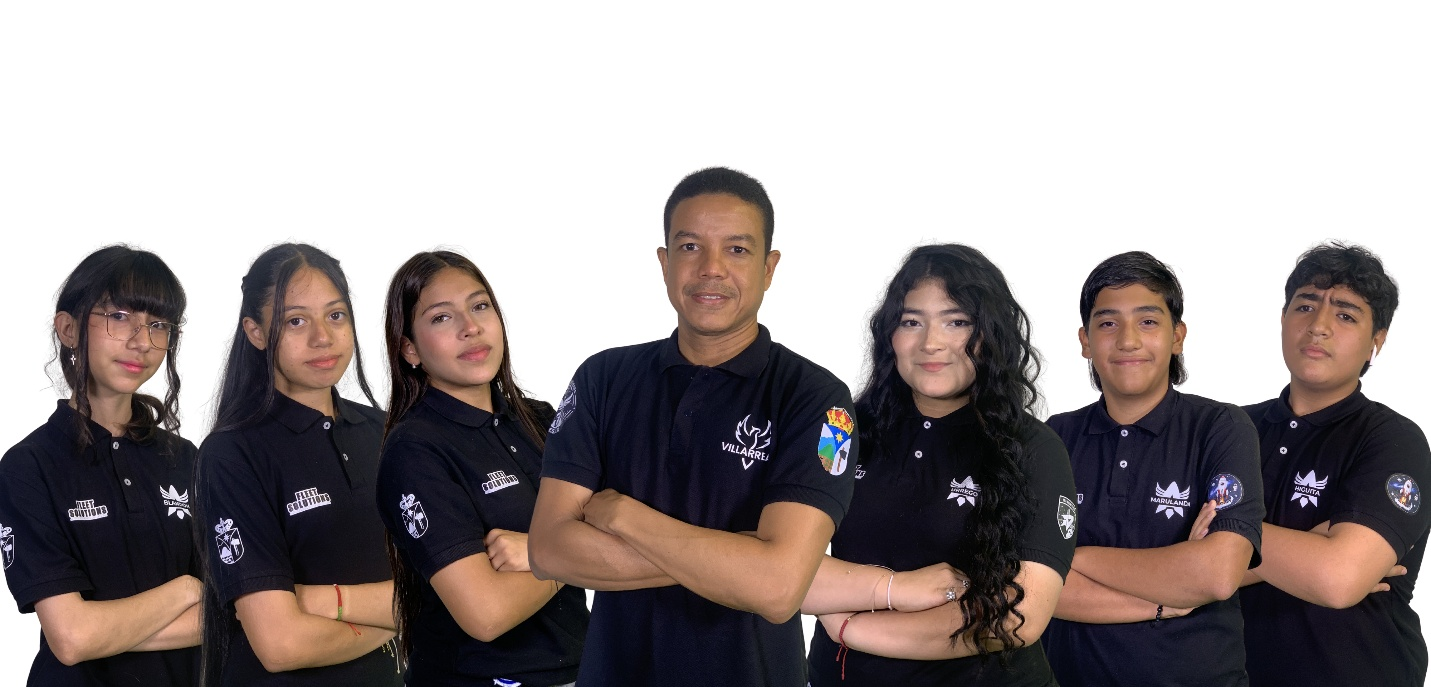
\includegraphics[width=0.75\linewidth]{equipo_mision.jpg}
\caption{Fotografía del equipo oficial PDA STARS (Equipo 211).}
\label{fig:equipo_mision}
\end{figure}

\subsection{Estructura Organizacional y Roles Técnicos}
\begin{table}[H]
\centering
\small
\begin{tabularx}{\linewidth}{p{4.2cm}p{3.5cm}X}
\toprule
\rowcolor{navyiejaga!15}
\textbf{Miembro / Rol} & \textbf{Responsabilidad Principal} & \textbf{Área Técnica Asignada} \\
\midrule
\textbf{Líder de Misión} & Samuel Gómez Correa & Coordinación general, cronograma de hitos, integración interdisciplinaria y vocería técnica. \\
\rowcolor{grisclaro}
\textbf{Diseño y Aerodinámica} & Responsable Técnico & Simulación digital OpenRocket, modelado CAD 3D de aletas y ojiva Haack, optimización del margen estático ($CG/CP$). \\
\textbf{Estructura y Materiales} & Responsable Técnico & Mecanizado de tubos Kraft BT-80, manufactura aditiva FDM en filamentos PETG/PETG-CF, acoples y ensamble estructural. \\
\rowcolor{grisclaro}
\textbf{Propulsión y Recuperación} & Responsable Técnico & Montaje del tubo portamotor 29 mm, cálculo de retardos, dimensionamiento del paracaídas ripstop de 40 cm y manta Nomex. \\
\textbf{Carga Útil y Aviónica} & Responsable Técnico & Programación de microcontrolador Seeeduino XIAO, integración de sensores DPS310/MPU6050, diseño PCB y telemetría. \\
\rowcolor{grisclaro}
\textbf{Oficial de Seguridad (RSO)} & Responsable Técnico & Verificación de listas de chequeo en rampa, inspección pre-vuelo, cumplimiento de radios de exclusión y gestión de riesgos. \\
\bottomrule
\end{tabularx}
\caption{Organigrama de responsabilidades del equipo PDA STARS.}
\label{tab:roles_equipo}
\end{table}
